\section{Die Gelfand-Dualität für topologische Mannigfaltigkeiten}\label{sec:GD2}

Mit dem Wissen, dass die Kategorie der kompakten Hausdorffräume dual zu der der \CAlgn{} ist, stellt sich nun die Frage, was passiert, wenn wir nur spezielle kompakte Hausdorffräume betrachten (also eine Unterkategorie). Konkret werden wir im Folgenden topologische Mannigfaltigkeiten betrachten und der Frage nachgehen, was wir über die zugehörigen \CAlgn{} sagen können.

\subsection{Vorüberlegungen}

\begin{defn}[kompakte topologische Mannigfaltigkeit]\label{defn:TopMan}
Ein kompakter Hausdorffraum $X$ heißt \emph{m-dimensionale kompakte topologische Mannigfaltigkeit}, wenn es stetige Abbildungen vom offenen Einheitsball $B^m$ aus $\RR^m$ nach $X$
\[ \theta_i: B^m \to X, ~i = 1, \dots, N \]
gibt (für ein $N \in \NN$), sodass gilt:
\begin{itemize}
	\item $\theta_i$ ist injektiv und $\theta_i^{-1}$ ist stetig sowie
	\item die Abbildung $\Theta: \bigcup_{i=1}^N(B^m,i) \to X: (r,i) \mapsto \theta_i(r)$ ist surjektiv.
\end{itemize}
Die Abbildungen $\theta_i$ bezeichnen wir als \emph{Karten}.
\end{defn}

\begin{prop}\label{prop:topManAlt}
Ist $X$ ein kompakter Hausdorffraum, so sind äquivalent:
\begin{enumerate}
	\item \label{prop:topManAlt:is}
		$X$ ist eine m-dimensionale kompakte topologische Mannigfaltigkeit.
	\item \label{prop:topManAlt:endl}
		Es gibt Abbildungen $\theta_i: B^m \to X$, sodass gilt:
		\begin{itemize}
			\item $\theta_i$ ist Homöomorphismus auf ihr Bild und
			\item $(\theta_i(B^m))_{i\in\{1,\dots,N\}}$ ist eine Überdeckung von $X$.
		\end{itemize}	\item \label{prop:topManAlt:pkt}
		Zu jedem $x \in X$ gibt es eine offene Umgebung $U_x \subseteq X$ von $x$ und einen Homöomorphismus $\theta_x: B^m \to U_x$, sodass $\theta_x(0) = x$.
	\item  \label{prop:topManAlt:abg}
		Es gibt Abbildungen $\theta_i: B^m \to X$, sodass gilt:
		\begin{itemize}
			\item $\theta_i$ ist Homöomorphismus auf ihr Bild und
			\item $(\theta_i(\overline{B_{0,5}^m}))_{i\in\{1,\dots,N\}}$ ist eine Überdeckung von $X$.
		\end{itemize}
\end{enumerate}
\end{prop}

\begin{proof}
\begin{itemize}
	\item[\ref*{prop:topManAlt:is}$\Rightarrow$\ref*{prop:topManAlt:endl}:] Die $\theta_i$ sind injektiv (also bijektiv auf ihr Bild) und stetig in beide Richtungen. Damit sind sie Homöomorphismen. Da $\Theta$ surjektiv ist, gibt es außerdem für jedes $x \in X$ ein $i \leq N$ und ein $r \in B^m$, sodass $x = \Theta(r,i) = \theta_i(r)$. Damit ist $(\theta_i(B^m))_{i\in\{1,\dots,N\}}$ eine Überdeckung.
	
	\item[\ref*{prop:topManAlt:is}$\Leftarrow$\ref*{prop:topManAlt:endl}:] Homöomorphismen sind insbesondere injektiv und in beide Richtungen stetig. Aus der Überdeckungseigenschaft folgt die Surjektivität von $\Theta$.
	
	\item[\ref*{prop:topManAlt:endl}$\Rightarrow$\ref*{prop:topManAlt:pkt}:] Sei $x \in X$. Da die $\theta_i(B^m)$ eine Überdeckung bilden, existiert ein $\theta_i$ mit $x \in \theta_i(B^m)$ und folglich $\theta_i^{-1}(x) \in B^m$. Weil $B^m$ offen ist, gibt es ein $\epsilon > 0$, sodass $B_\epsilon^m(\theta_i^{-1}(x)) \subseteq B^m$. Damit ist $U_x := \theta_i(B_\epsilon^m(\theta_i^{-1}(x)))$ eine offene Umgebung von $x$. Ferner ist die Abbildung
	\[\tau: B^m \to B_\epsilon^m(\theta_i^{-1}(x)): r \mapsto  \epsilon r + \theta_i^{-1}(x)\]
ein Homöomprphismus mit $\tau(0) = \theta_i^{-1}(x)$. Also ist $\theta_x := \theta_i \circ \tau: B^m \to U_x$ ein Homöomorphismus mit $\theta_x(0) = \theta_i \circ \tau(0) = \theta_i(\theta_i^{-1}(x)) = x$.
	
	\item[\ref*{prop:topManAlt:pkt}$\Rightarrow$\ref*{prop:topManAlt:abg}:] $(\theta_x(B_{0,5}^m))_{x\in X}$ ist Überdeckung von $X$. Da $X$ kompakt ist, gibt es also eine endliche Menge $M \subseteq X$, sodass auch $(\theta_x(B_{0,5}^m))_{x\in M}$ eine Überdeckung ist. Damit ist insbesondere auch $(\theta_x(\overline{B_{0,5}^m}))_{x\in M}$ eine Überdeckung von $X$ und es ist gezeigt, dass diese (endlich vielen) Abbildungen $\theta_x$ (für $x \in M$) die Anforderungen aus \ref*{prop:topManAlt:abg} erfüllen.

	\item[\ref*{prop:topManAlt:abg}$\Rightarrow$\ref*{prop:topManAlt:endl}:]Karten, die die Anforderungen aus \ref*{prop:topManAlt:abg} erfüllen, erfüllen offensichtlich insbesondere auch die aus \ref*{prop:topManAlt:endl}.	
\end{itemize}
\end{proof}

\begin{bem}
\cref*{prop:topManAlt:pkt} entspricht der üblichen Definition für kompakte topologische Mannigfaltigkeiten (die auch zur Definition von nicht notwendig kompakten topologischen Mannigfaltigkeiten verwendet wird).
\end{bem}

Die Klasse aller \komenTopMan{} mit stetigen Abbildungen als Morphismen bildet die \emph{Kategorie der kompakten topologischen Mannigfaltigkeiten} $\KatTopMan$. Da jede \komTopMan{} auch ein kompakter Hausdorffraum ist, ist $\KatTopMan$ offensichtlich eine Unterkategorie von $\KatTop$. 

Aufgrund der Gelfand-Dualität muss es folglich eine zu $\KatTopMan$ duale Unterkategorie von $\KatCAlg$ geben. Wir werden diese Kategorie als \emph{Kategorie der \CAlgMann} $\KatCAlgMan$ bezeichnen und im Folgenden versuchen die Objekte dieser Kategorie näher zu klassifizieren. Wir werden also versuchen die Frage zu beantworten, welche \CAlgn{} isomorph zum Raum der stetigen Funktionen über einer \komenTopMan{} sind.

Betrachten wir dazu eine \komTopMan{} $X$ mit Karten $\theta_i$. Über die Gelfand-Dualität erhalten wir zu $X$ die \CAlg{} $\stetig(X)$. Weiterhin erhalten wir aus den Karten von $X$ auf natürliche Weise stetige Algebrenhomomorphismen 
	\[k_i: \stetig(X) \to \stetig^b(B^m):= \{\varphi: B^m \to \CC ~|~ \varphi \text{ stetig und beschränkt}\}: \tau \mapsto \tau \circ\theta_i.\]
Die Eigenschaft solche \glqq Karten\grqq{} zu besitzen, bleibt offensichtlich unter Isomorphie erhalten (verknüpfe die Abbildungen mit dem Isomorphismus). Also müssen alle \CAlgn{} der Unterkategorie $\KatCAlgMan$ derartige \glqq Karten\grqq{} besitzen (wir werden diese im Folgenden als \emph{Algebrenkarten} bezeichnen). 

Nun sind die Karten einer \komTopMan{} jedoch nicht beliebige stetige Abbildungen, sondern sie besitzen zusätzlich noch eine Injektivitäts- und eine Surjektivitätseigenschaft. Diese Eigenschaften der Karten sollten sich in irgendeiner Weise auch in den Algebrenkarten widerspiegeln. 

Tatsächlich ist leicht zu sehen, dass sich aus der Surjektivität von $\Theta$, die Injektivität der Abbildung
	\[K: \stetig(X) \to (\stetig^b(B^m))^N: \tau \mapsto (\tau\circ\theta_1, \dots, \tau\circ\theta_N)\]
ergibt. 

Analog könnte man vielleicht erwarten, dass aus der Injektivität der Karten $\theta_i$ folgt, dass die Algebrenkarten $k_i$ surjektiv sind. Dass dies jedoch nicht der Fall ist, können wir an folgenden Beispiel sehen:

\begin{bsp}\label{bsp:ohneNS} $S^1 := \{z \in \CC ~|~ |z| = 1\}$ ist ein kompakter Hausdorffraum, der mit den Karten 
	\[\theta_{\hat{N}}: B^1 \to S^1: r \mapsto \exp{\pi i r - 0,5\pi i} \text{ und } \theta_{\hat{S}}: B^1 \to S^1: r \mapsto \exp{\pi i r + 0,5\pi i}\]
vollständig überdeckt wird. Also ist $S^1$ eine topologische Mannigfaltigkeit. Ferner ist die Abbildung:
	\[\varphi: B^1 \to \CC: r \mapsto r\]
offensichtlich stetig und beschränkt, d.h. $\varphi \in \stetig^b(B^1)$.

Wäre nun $k_{\hat{N}}: \stetig(S^1) \to \stetig^b(B^1): \tau \mapsto \tau \circ\theta_{\hat{N}}$ surjektiv, so müsste es eine Abbildung $\tau \in \stetig(S^1)$ geben, die auf $\varphi$ abgebildet wird. Dieses $\tau$ müsste dann aber direkt \glqq rechts\grqq{} von Nordpol fast $1$ und direkt \glqq links\grqq{} fast $-1$ sein - da $\tau$ stetig sein soll, hieße das:
	\begin{align*}
		1 &= \lim_{r\to 1}\varphi(r) = \lim_{r\to 1} \tau\circ\theta_{\hat{N}}(r) = \lim_{r\to 1}\tau(\exp{\pi i r - 0,5\pi i}) =  \tau(\exp{0,5\pi i}) = \\
		 &=\tau(\exp{-1,5\pi i}) = \lim_{r\to -1} \tau(\pi i r - 0,5\pi i) = \lim_{r\to -1} \tau\circ\theta_{\hat{N}}(r) = \lim_{r\to -1}\varphi(r) = -1
	\end{align*}
Also gibt es kein solches $\varphi$ und $k_{\hat{N}}$ ist nicht surjektiv.
\end{bsp}

\begin{figure}[h]
         \centering
         \begin{subfigure}[b]{0.3\textwidth}
                 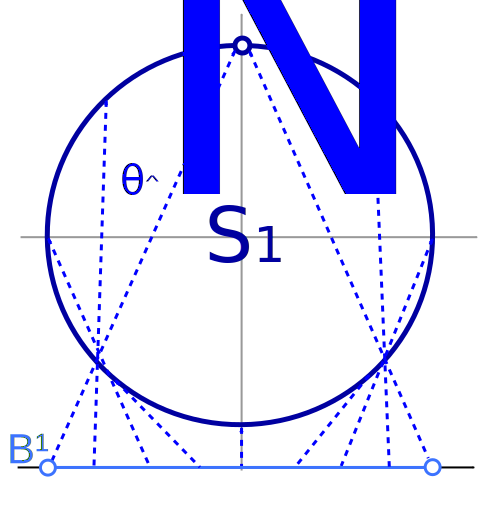
\includegraphics[width=\textwidth]{Bilder/keine-ueberdeckung.pdf}
                 \caption{\Cref{bsp:ohneNS}}
         \end{subfigure}%
 			\qquad\qquad
         \begin{subfigure}[b]{0.3\textwidth}
                 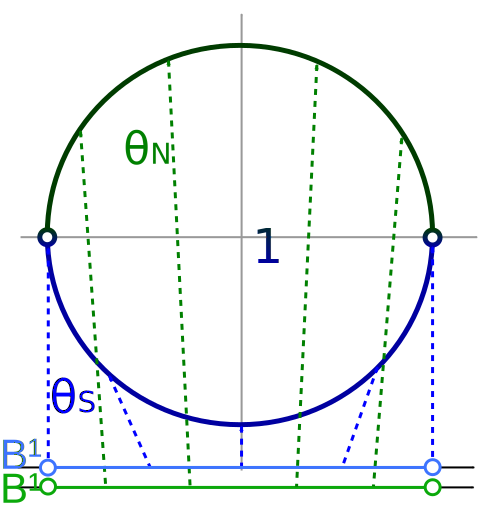
\includegraphics[width=\textwidth]{Bilder/ohne-aequator.pdf}
                 \caption{\Cref{bsp:keine-Ueberdeckung}}
         \end{subfigure}
         \caption{Kartenabbildungen für $S^1$}
\end{figure}

Ein weiteres Problem ist, dass aus der Surjektivität von $\Theta$ zwar die Injektivität von $K$ folgt, nicht aber umgekehrt:

\begin{bsp}\label{bsp:keine-Ueberdeckung}Die Karten 
	\[\theta_S: B^1 \to S^1: r \mapsto \exp{0,5 \pi i (r-1)} \text{ und } \theta_N: B^1 \to S^1: r \mapsto \exp{0,5 \pi i (1-r)}\]
bilden keine vollständige Überdeckung von $S^1$ (die beiden Äquatorpunkte werden nicht getroffen). Dennoch wäre $K$ zu diesen Karten bereits injektiv. Denn gilt für zwei Abbildungen $\tau, \psi \in \stetig(S^1)$, dass $(\tau\circ\theta_S, \tau\circ\theta_N) = K(\tau) = K(\psi) = (\psi\circ\theta_S, \psi\circ\theta_N)$ ist, so können sich $\tau$ und $\psi$ höchstens noch an den Äquatorpunkten unterscheiden. Da $\tau$ und $\psi$ aber stetig sind, sind diese beiden Punkte bereits durch ihre Umgebung eindeutig festgelegt. Folglich müssen $\tau$ und $\psi$ auch hier übereinstimmen und sind damit identisch.
\end{bsp}

Insgesamt sehen wir also, dass die Surjektivität der Algebrenkarten eine zu starke Forderung ist, während die Injektivität von $K$ anscheinend eine zu schwache Bedingung ist. 

\subsection{Satz und Beweis}

Der Versuch die in den Vorüberlegungen aufgetauchten Probleme zu beseitigen, führt uns zu der folgenden Charakterisierung von \CAlgMann.

\begin{defn}[kompakte Konvergenz]\label{defn:komKonv}
Sei ein topologischer Raum $X$ und eine Folge von Funktionen $(\psi_l: X \to \CC)_{l \in \NN}$ gegeben. Diese Folge \emph{konvergiert kompakt} gegen eine Funktion $\psi: X \to \CC$, wenn die Folge auf jeder kompakten Teilmenge von $X$ gleichmäßig gegen $\psi$ konvergiert.
\end{defn}

\begin{defn}[\CAlgMann]\label{defn:CAM}
Eine \CAlg{} $\A$ heißt \emph{\CAlgMan{} der Dimension $m$}, wenn es stetige Algebrenhomomorphismen
	\[k_i: \A \to \stetig^b(B^m), ~i = 1, \dots , N\]
gibt (für ein $N \in N$), sodass gilt:
\begin{defenum}
	\item \label{defn:CAM:surj}
	Zu allen $i \leq N$ und $\psi \in \stetig(\overline{B^m})$ mit $\psi|_{\partial B^m} \equiv \mathrm{const.}$ gibt es ein $a \in \A$, sodass $k_i(a) = \psi|_{B^n}$.
	\item \label{defn:CAM:kompkonv}
	Sind $(a_l)_{l \in \mathbb{N}} \subset \A$ und $\psi_i \in \stetig(B^m)$ mit
	\[\forall i: k_i(a_l) \overset{l \to \infty}{\longrightarrow} \psi_i \text{ konvergiert kompakt,}\]
	dann $\exists a \in \A: a_l \overset{l \to \infty}{\longrightarrow} a$ (Konvergenz in $\A$).
\end{defenum}
Diese Abbildungen bezeichnen wir als \emph{Algebrenkarten}.
\end{defn}

\begin{bem}
\ref{defn:CAM:surj} ist eine Art abgeschwächte Surjektivität: Es muss nämlich nur eine bestimmte Teilmenge der stetigen Abbildungen auf $\overline{B^m}$ getroffen werden. Die Einschränkung auf Abbildungen, die auf dem Rand konstant sind, verhindert gerade das Problem aus \Cref{bsp:ohneNS}.

Entsprechend unterbindet \ref{defn:CAM:kompkonv} das Problem aus \Cref{bsp:keine-Ueberdeckung} (wähle dazu eine Folge von Abbildungen in $\stetig(S^1)$, die gegen eine Abbildung konvergiert, die gerade an den beiden Äquatorpunkten Polstellen besitzt). Diese Eigenschaft ist dabei eine stärkere Forderung als die bloße Injektivität von $K$, d.h. die Injektivität dieser Abbildung folgt aus \ref*{defn:CAM:kompkonv}: Sind nämlich $a,b \in \A$, sodass für alle $i \leq N$ gilt $k_i(a) = k_i(b)$, dann ist $(k_i(a), k_i(b), k_i(a), k_i(b), \dots)$ eine konstante Folge und damit (kompakt) konvergent. Nach \ref*{defn:CAM:kompkonv} konvergiert dann auch $(a, b, a, b, \dots)$ in $\A$ und somit muss $a = b$ gelten.
\end{bem}

\begin{bem}
Die Dimension $m$ einer \CAlgMan{} $\A$ ist nicht identisch zu der Dimension $n$, die $\A$ als Vektorraum bzw. \CAlg{} besitzt. Allerdings werden wir sehen, dass sowieso immer nur einer der beiden Dimensionsbegriffe von Interesse ist. 

Ist nämlich die Dimension einer \CAlgMan{} $\A$ größer als $0$, so auch die der zugehörigen topologischen Mannigfaltigkeit $\SpecC(\A)$ (siehe den Beweis zu \Cref{satz:GD2}). Dann kann $\SpecC(\A)$ aber keine endliche Menge sein und daher $\A$ nach \Cref{sec:Anwendung} als \CAlg{} nicht mehr endlich dimensional. Ist umgekehrt die Dimension von $\A$ als \CAlg{} endlich, so muss die Dimension von $\A$ als \CAlgMan{} bereits $0$ sein.
\end{bem}

\begin{satz}[Gelfand-Dualität für \komenTopMan]\label{satz:GD2}
Die Kategorie der kompakten topologischen Mannigfaltigkeiten $\KatTopMan$ ist dual zu der der \CAlgMann{} $\KatCAlgMan$.
\end{satz}

\begin{proof}Wir verwenden hier die gleichen Funktoren wie in der gewöhnlichen Gelfand-Dualität (\Cref{satz:GD}):
	\[\begin{array}{@{}rrcl@{}}
	 			&\KatTopMan			&\simeq		&\KatCAlgMan^\op 												\\
	\stetig: 	&X					&\mapsto	&\stetig(X)													\\
				&(\varphi:X \to Y)	&\mapsto	&(h_\varphi: \stetig(Y) \to \stetig(X): \tau \mapsto \tau \circ \varphi)^\op 		\\
	\SpecC:		&\SpecC(\A)													&\mapsfrom	&\A				\\
				&(\varphi_h: \SpecC(\A) \to \SpecC(\B): f \mapsto f \circ h)	&\mapsfrom	&(h: \B \to \A)^\op
	\end{array}\]
Nun ist jede \komTopMan{} auch ein kompakter Hausdorffraum und zwei \komenTopMan{} sind isomorph genau dann, wenn sie es als kompakte Hausdorffräume sind (da beide Kategorien die gleichen Morphismen besitzen). Analog ist jede \CAlgMan{} auch eine \CAlg{} und zwei \CAlgMann{} sind isomorph genau dann, wenn sie es als \CAlgn{} sind. Die Dualität der Kategorien folgt also im Wesentlichen schon aus der gewöhnlichen Gelfand-Dualität (\Cref{satz:GD}).

Zu zeigen ist allerdings noch, dass die Funktoren in obiger Form überhaupt wohldefiniert sind, das heißt, dass $\stetig$ jeder \komenTopMan{} eine \CAlgMan{} zuordnet und umgekehrt $\SpecC$ jeder \CAlgMan{} eine \komTopMan{}.

Sei dazu zunächst $X$ eine \komTopMan{}. Dann gibt es nach \Cref{prop:topManAlt} Karten $\theta_i: B^m \to X$, sodass $(\theta_i(\overline{B_{0,5}^m}))_{i=1,\dots,N}$ eine Überdeckung von $X$ bilden. Daraus  definieren wir uns wie folgt Algebrenkarten:
	\[k_i: \stetig(X) \to \stetig^b(B^m): \tau \mapsto \tau \circ \theta_i \]
Zu zeigen ist nun also:
\begin{proofenum}
	\item \label{proof:GD2:kAlghom}
		Die $k_i$ sind stetige Algebrenhomomorphismen.
	\item \label{proof:GD2:schwachsurj}
		Zu allen $i \leq N$ und $\psi \in \stetig(\overline{B^m})$ mit $\psi|_{\partial B^m} \equiv \mathrm{const.}$ gibt es ein $\tau \in \stetig(B^m)$, sodass $k_i(\tau) = \psi|_{B^m}$.
	\item \label{proof:GD2:komkonv}
		Sind $(\tau_l)_{l \in \NN} \subset \stetig(X)$ und $\psi_i \in \stetig(B^m)$ so, dass
			\[\forall i: k_i(\tau_l) \overset{l \to \infty}{\longrightarrow} \psi_i \text{ kompakt konvergiert,}\]
		dann $\exists \tau \in \stetig(X): \tau_l \overset{l \to \infty}{\longrightarrow} \tau$.
	\setcounter{temp}{\value{proofenumi}}
\end{proofenum}

Zu \ref{proof:GD2:kAlghom}: Dass $k_i$ ein Algebrenhomomorphismus ist, zeigt sich durch einfaches Nachrechnen der entsprechenden Axiome. Für die Stetigkeit sei $\tau \in \stetig(X), ~\epsilon > 0$, dann gilt für alle $\psi \in \stetig(X)$ mit $\norm{\tau - \psi} < \epsilon $:
\begin{align*}
\norm{k_i(\tau)-k_i(\psi)} &= \norm{\tau \circ \theta_i - \psi \circ \theta_i} = \underset{r \in B^m}{\sup} |\tau \circ \theta_i(r) - \psi \circ \theta_i(r)| \\
 &\leq \underset{x \in X}{\sup} |\tau (x) - \psi (x)| = \norm{\tau- \psi} < \epsilon
\end{align*}
Also ist $k_i$ ein stetiger Algebrenhomomorphismus.

Zu \ref{proof:GD2:schwachsurj}: Sei $\psi \in \stetig(\overline{B^m} )$ mit $\psi|_{\partial B^m} \equiv \lambda \in \mathbb{C}$ und $i \leq N$. Dann definiere:
\[\tau: X \to \CC: x \mapsto \begin{cases} \psi(\theta_i^{-1}(x)) &, x \in \theta_i(B^m) \\ \lambda &, \text{ sonst} \end{cases} \]
Diese Abbildung hat die gewünschte Eigenschaft:
\[k_i(\tau) = \tau \circ \theta_i = \psi \circ \theta_i^{-1} \circ \theta_i = \psi|_{B^m}\]
Noch zu zeigen ist, dass $\tau$ auch tatsächlich stetig ist. Dazu sei $x \in X$ und $\epsilon > 0$ beliebig.
\Fall{1} $x \in \theta_i(B^m)$ bzw. $\theta^{-1}(x) \in B^m$

Da $\psi$ stetig ist, existiert ein $\delta > 0$, sodass gilt: 
	\[\forall r \in B^m: \norm{r - \theta_i^{-1}(x)} <\delta \Rightarrow \left|\psi(r) - \psi(\theta_i^{-1}(x))\right| < \epsilon \]
Dann ist $\theta_i\left(B_\delta^m(\theta_i^{-1}(x)) \cap B^m\right) \subseteq X$ eine offene Umgebung von $x$ und es gilt für alle $y \in \theta_i\left(B_\delta^m(\theta_i^{-1}(x)) \cap B^m\right)$, dass $\theta_i^{-1}(y) \in B_\delta^m(\theta_i^{-1}(x))$, also
	\[\left|\tau(y) - \tau(x)\right| = \left|\psi(\theta_i^{-1}(y)) - \psi(\theta_i^{-1}(x))\right| < \epsilon.\]

\Fall{2} $x \notin \theta_i(B^m)$, d.h. $\tau(x) = \lambda$.

Da $\psi \in \stetig(\overline{B^m})$ ist, gibt es insbesondere für alle $r \in \partial B^m$ ein $\delta_r > 0 $, sodass
	\[\forall s \in B_{\delta_r}^m(r) \cap \overline{B^m}: |\psi(s) - \lambda| = |\psi(s) - \psi(r)| < \epsilon.\]
Nun ist $U := \bigcup_{r \in \partial B^m}B_{\delta_r}^m(r) \supseteq \partial B^m$ offen und daher $\overline{B^m} \backslash U$ und $\theta_i\left(\overline{B^m} \backslash U\right)$ abgeschlossen. Folglich ist $X \backslash \theta_i\left(\overline{B^m} \backslash U\right) \supset X \backslash \theta_i(\overline{B^m})$ eine offene Umgebung von $x$ und es gilt:
	\[\forall y \in X \backslash \theta_i\left(\overline{B^m} \backslash U\right): \left|\psi(y) - \psi(x)\right| = \begin{cases} |\psi(\theta_i^{-1}(y)) - \lambda| < \epsilon &, y \in U \cap \overline{B^m} \\ |\lambda - \lambda| = 0 < \epsilon &, \text{ sonst}\end{cases}\]
In beiden Fällen ist $\tau$ also stetig.

Zu \ref{proof:GD2:komkonv}: Seien $ (\tau_l)_{l\in \mathbb{N}} \subset \stetig(X), ~\psi_i \in \stetig(B^m)$ so, dass
\[\forall i: k_i(\tau_l) \overset{l \to \infty}{\longrightarrow} \psi_i ~\text{kompakt konvergiert.}\]
Dann definiere:
\[\tau: X \to \mathbb{C}: x \mapsto \psi_i(r), \text{ mit } r\in B^m \text{ und } i\in \{1,\dots,N\} \text{ so, dass } \theta_i(r) = x \]
Dies ist wohldefiniert, denn
\begin{itemize}
  \item $(\theta_i(B^m))_{i\in\{1,\dots,N\}}$ ist Überdeckung von $X$, also können $i$ und $r$ wie verlangt gewählt werden.
  \item Seien $i,j \in \{1,\dots,N\}$ und $r,s \in B^m$ so, dass $\theta_i(r) = x = \theta_j(s)$. Dann gilt (da $\{r\}, \{s\} \subset B^m$ kompakt):
  \[\psi_i(r) = \underset{l \to \infty}{\lim} \tau_l\circ\theta_i(r) = \underset{l \to \infty}{\lim} \tau_l (x) = \underset{l \to \infty}{\lim} \tau_l\circ\theta_j(s) = \psi_j(s)\]
\end{itemize}

Ferner ist $\tau$ stetig, denn für jedes $x \in X$ gibt es eine offene Umgebung $B_\epsilon^m(\theta_i^{-1}(x)) \subseteq B^m$ von $\theta_i^{-1}(x)$ und damit eine offene Umgebung $\theta_i(B_\epsilon^m(\theta_i^{-1}(x)))$ von $x$. Auf dieser ist $\tau$ identisch zu $\psi \circ \theta_i^{-1}$, welches eine stetige Abbildung ist. Also ist $\tau$ stetig in $x$ und entsprechend auf ganz $X$.

Noch zu zeigen ist, dass die $\tau_l$ gleichmäßig gegen $\tau$ konvergieren. Da für jedes $i \leq N$ die $k_i(\tau_l)$ kompakt gegen $\psi_i$ konvergieren, konvergieren diese auf der kompakten Menge $\overline{B_{0,5}^m}$ gleichmäßig. Das heißt für jedes $\epsilon > 0$ gibt es ein $L_i \in \NN$, sodass
	\[\forall l \geq L_i, r \in \overline{B_{0,5}^m}: \left| k_i(\tau_l)(r) - \psi_i(r) \right| < \epsilon.\]
Also gilt für $L := \max\{L_1, \dots, L_N\}$ und alle $i \leq N$:
	\[\forall l \geq L, r \in \overline{B_{0,5}^m}: \left|\tau_l(\theta_i(r)) - \tau(\theta_i(r))\right| = \left|k_i(\tau_l)(r) - \psi(r)\right|  < \epsilon\]
Aus $\bigcup_{i=1}^N\theta_i(\overline{B_{0,5}^m}) = X$ folgt damit, dass die $\tau_l$ auf ganz $X$ gleichmäßig gegen $\tau$ konvergieren. Also ist $\tau \in \stetig(X)$ und $\tau_l \overset{l \to \infty}{\longrightarrow} \tau$.

Insgesamt folgt aus \ref{proof:GD2:kAlghom}, \ref{proof:GD2:schwachsurj} und \ref{proof:GD2:komkonv}, dass die $k_i$ tatsächlich Algebrenkarten sind und $\stetig(X)$ somit eine \CAlgMan{} ist.


Bleibt noch die andere Richtung: Sei dazu $\A$ eine \CAlgMan{}. Dann gibt es Algebrenkarten $k_i: \A \to \stetig^b(B^m)$. Daraus  definieren wir uns nun Karten für $\SpecC(\A)$:
	\[\theta_i: B^m \to \SpecC(\A): r \mapsto (f_r^i: \A \to \CC: a \mapsto k_i(a)(r)) \]
Zu zeigen ist jetzt:
\begin{proofenum}
	\setcounter{proofenumi}{\value{temp}}
	\item \label{proof:GD2:fAlghom}
		Die $f_r^i$ sind stetige Algebrenhomomorphismen.
	\item \label{proof:GD2:Homoeo}
		Die $\theta_i$ sind Homöomorphismen auf ihr Bild.
	\item \label{proof:GD2:Ueberdeckung}
		$(\theta_i(B^m))_{i\in\{1,\dots,N\}}$ ist eine Überdeckung von $\SpecC(\A)$.
\end{proofenum}
Dann ist $\SpecC(\A)$ nach \Cref{prop:topManAlt} eine \komTopMan.

Zu \ref{proof:GD2:fAlghom}: Dass $f_r^i$ ein Algebrenhomomorphismus ist, ergibt sich wieder durch Nachrechnen der Axiome. Zum Beweis der Stetigkeit sei $a \in \A$ und $\epsilon > 0$. Dann gibt es, da $k_i$ stetig, ein $\delta>0$ sodass 
\[\forall b \in \A: \norm{a-b} < \delta \Rightarrow \norm{k_i(a)-k_i(b)} < \epsilon\]
Damit gilt $\forall b \in \A$ mit $\norm{a-b} < \delta$
\[ |f_r^i(a) - f_r^i(b)| = |k_i(a)(r)-k_i(b)(r)| \leq \underset{s \in B^m}{\sup} |k_i(a)(s)-k_i(b)(s)| = \norm{k_i(a)-k_i(b)} < \epsilon\]
Also ist $f_r^i$ ein stetiger Algebrenhomomorphismus.

Zu \ref{proof:GD2:Homoeo}: \begin{itemize}
	\item $\theta_i$ ist injektiv, denn:
	
	Seien $r, s \in B^m$ mit $\theta_i(r) = \theta_i(s)$, d.h. 
	\begin{align*}
		\forall a \in \A: k_i(a)(r) = f_r^i(a) = \theta_i(r)(a) = \theta_i(s)(a) = f_s^i(a)  = k_i(a)(s)
	\end{align*}
	Angenommen es wäre $r \neq s$. Dann gäbe es nach dem Lemma von Urysohn ein stetiges $\psi: \overline{B^m} \to \mathbb{C}$ mit
	\[\psi|_{\partial B^m \cup \{r\}} \equiv 0, ~\psi(s) = 1\]
	Da $\A$ eine \CAlgMan{} ist, gibt es ein $a \in \A: k_i(a) = \psi|_{B^m}$. Also gilt 
	\[\theta_i(r)(a) = k_i(a)(r) = \psi(r) = 0 \neq 1 = \psi(s) = k_i(a)(s) = \theta_i(s)(a),\]
	was im Widerspruch zur Voraussetzung $\theta_i(r) = \theta_i(s)$ steht. Daher ist doch $r = s$.
	
	\item $\theta_i$ ist stetig, denn:
	
	Seien $r \in B^m, \epsilon > 0$ und $a \in \A$, also
	\[U_i(f_r^i, a, \epsilon) := \{f_s^i \in \theta_i(B^m) ~\big|~ |f_r^i(a) - f_s^i(a)| < \epsilon\}\]
	eine offene Umgebung von $f_r^i$. Dann ist $k_i(a) \in \stetig^b(B^m)$, d.h. 
	\[\exists \delta >0: \forall s \in B^m: |r-s| <\delta \Rightarrow |k_i(a)(r) - k_i(a)(s)| < \epsilon\]
	Damit gilt für alle $s \in B^m$ mit $|r-s| < \delta$:
	\[ |f_r^i(a) - f_s^i(a)| = |k_i(a)(r) - k_i(a)(s)| < \epsilon \]
	also $\theta_i(s) = f_s^i \in U_i(f_r^i, a, \epsilon)$.
	
	\item $(\theta_i|_{\theta_i(B^m)})^{-1}$ ist stetig, denn:
	
	Sei $f_r^i \in \theta_i(B^m), \epsilon>0$ (oBdA sei $\epsilon$ so klein, dass $B_\epsilon^m(r) \subset B^m$). Dann gibt es nach dem Lemma von Urysohn eine stetige Funktion
	\[\psi: \overline{B^m} \to \mathbb{C} \text{ mit } \psi|_{\overline{B^m}\backslash B_\epsilon^m(r)} \equiv 0, ~\psi(r) = 1\]
	Da $\A$ eine \CAlgMan{} ist, gibt es ein $a \in \A$ mit $k_i(a) = \psi|_{B^m}$.
	
	Damit gilt für alle $f_s^i \in U_i(f_r^i, a, 1)$:
	\[|1 - \psi(s)| = |\psi(r) - \psi(s)| = |\theta_i(a)(r) - \theta_i(a)(s)| = |f_r^i(a) - f_s^i(a)| < 1\]
	Also $\psi(s) \neq 0$ und damit nach Definition von $\psi$:
	\[s \notin \overline{B^m}\backslash B_\epsilon(r) \Rightarrow s \in B_\epsilon^m(r) \Rightarrow |r-s| < \epsilon\]
\end{itemize}
Damit ist $\theta_i$ ein Homöomorphismus auf ihr Bild.

Zu \ref{proof:GD2:Ueberdeckung}: \Ann $\exists f \in \SpecC(\A) \backslash \bigcup_{i=1}^N \theta_i(B^m)$.

Dann definiere 
\[W_l := \bigcup_{i=1}^N \theta_i(\overline{B_{1-\frac{1}{l}}(0)}) \subset \bigcup_{i=1}^N \theta_i(B^m)\]
Die $W_l$ sind als endliche Vereinigung abgeschlossener Mengen ebenfalls abgeschlossen. Damit existieren dem Lemma von Urysohn zu Folge ($\SpecC(\A)$ ist ein kompakter Hausdorffraum) stetige Funktionen
\[\psi_l: \SpecC(\A) \to \mathbb{C} \text{ mit } \psi_l|_{W_l} \equiv 0, ~\psi_l(f) = l.\]
Nun sind die $\psi_l \in \stetig(\SpecC(\A))$, welcher laut Satz von Gelfand-Neumark (\Cref{satz:GN}) isometrisch isomorph zu $\A$ ist. Nach Definition des Isomorphismuses $\AlgIso: \A \to  \stetig(\SpecC(\A))$ gibt es damit $a_l \in \A$, sodass:
\[\psi_l = \AlgIso(a_l) = \tau_{a_l}: f \mapsto f(a_l)\]
Ferner gilt für $r \in \overline{B_{1-\frac{1}{l}}^m(0)}$:
\[k_i(a_l)(r) = f_r^i(a_l) = \tau_{a_l}(f_r^i) = \psi_l(f_r^i) = \psi_l(\theta_i(r)) = 0\]
Sei $W \subset B^m$ kompakt, dann gibt es ein $L \in \mathbb{N}$, sodass $W \subset \overline{B_{1-\frac{1}{L}}^m(0)}$ und damit:
\[\forall l \geq L: W \subset \overline{B_{1-\frac{1}{l}}^m(0)} \text{, d.h. } k_i(a_l)|_W \equiv 0\]
Also konvergiert $k_i(a_l)$ kompakt gegen die Nullfunktion auf $\stetig(B^m)$ und es gibt ein $a \in \A$ mit $a_l \overset{l \to \infty}{\longrightarrow} a$. Folglich muss es auch ein $\psi \in \stetig(\SpecC(\A))$ geben, sodass $\psi_l \overset{l \to \infty}{\longrightarrow} \psi$. Für dieses gilt dann:
\[|l - \psi(f)| = |\psi_l(f) - \psi(f)| \leq \underset{g \in \SpecC(\A)}{\sup}|\psi_l(g) - h(g)| \overset{l \to \infty}{\longrightarrow} 0 \]
Also $|l - \psi(f)| \overset{l \to \infty}{\longrightarrow} 0$ und damit $\psi(f) = \infty ~\lightning$

Daher muss die Annahme falsch sein und doch $\SpecC(\A) = \bigcup_{i=1}^N \theta_i(B^m)$ gelten, d.h. $(\theta_i(B^m))_{i=1,\dots,N}$ eine Überdeckung von $\SpecC(\A)$ sein.

Aus \ref{proof:GD2:fAlghom}, \ref{proof:GD2:Homoeo} und \ref{proof:GD2:Ueberdeckung} folgt jetzt, dass $\SpecC(\A)$ eine topologische Mannigfaltigkeit ist. Damit ist die Wohldefiniertheit der Funktoren $\stetig$ und $\SpecC$ für \Cref{satz:GD2} gezeigt.
\end{proof}

Diese Erweiterung der Gelfand-Dualität für \komTopMann{} bestätigt nun, dass wir mit den in \Cref{defn:CAM} definierten \CAlgMann{} tatsächlich eine Klassifikation der zu $\KatTopMan$ dualen Kategorie $\KatCAlgMan$ gefunden haben. Können wir also für eine \CAlg{} zeigen, dass sie zusätzlich die Eigenschaften einer \CAlgMan{} besitzt (d.h. es entsprechende Algebrenkarten gibt), dann wissen wir bereits, dass der ihr durch die Gelfand-Dualität zugeordnete kompakte Hausdorffraum eine topologische Mannigfaltigkeit ist.